% Presentation deck for the paper — a guided walkthrough of the problem,
% the method, and the tool, ending in the community call to action.
% Build: make slides   (pdflatex twice; screenshots come from ../docs/screenshots
% via the `assets` target, which converts the SVGs with inkscape).
% Landscape 16:9, themed to match the report's dark palette (scales.py/render.py).
\documentclass[aspectratio=169,10pt]{beamer}

\usepackage[utf8]{inputenc}
\usepackage[T1]{fontenc}
\usepackage[scaled=0.92]{helvet}
\usepackage{microtype}
\usepackage{tikz}
\usetikzlibrary{positioning,patterns,arrows.meta}
\usepackage{pgfplots}
\pgfplotsset{compat=1.18}
\usepackage{qrcode}
\usepackage{graphicx}
\graphicspath{{assets/}}

\usetheme[progressbar=frametitle,numbering=fraction,block=fill]{metropolis}

% ---- palette: the report's own dark theme -------------------------------
\definecolor{SlideBg}{HTML}{1A1C19}
\definecolor{Panel}{HTML}{22241F}
\definecolor{PanelHi}{HTML}{2A2C27}
\definecolor{Ink}{HTML}{EFE9DA}
\definecolor{InkSoft}{HTML}{B7B4A6}
\definecolor{InkFaint}{HTML}{8B8D80}
\definecolor{Sage}{HTML}{6C9A8B}
\definecolor{Tan}{HTML}{C5B48A}
\definecolor{Amber}{HTML}{D99058}
\definecolor{Rust}{HTML}{B04A3A}

\setbeamercolor{normal text}{fg=Ink,bg=SlideBg}
\setbeamercolor{frametitle}{fg=Ink,bg=Panel}
\setbeamercolor{progress bar}{fg=Sage,bg=PanelHi}
\setbeamercolor{title separator}{fg=Sage}
\setbeamercolor{progress bar in head/foot}{fg=Sage,bg=PanelHi}
\setbeamercolor{progress bar in section page}{fg=Sage,bg=PanelHi}
\setbeamercolor{alerted text}{fg=Amber}
\setbeamercolor{example text}{fg=Sage}
\setbeamercolor{itemize item}{fg=Sage}
\setbeamercolor{itemize subitem}{fg=Sage}
\setbeamercolor{enumerate item}{fg=Sage}
\setbeamercolor{page number in head/foot}{fg=InkFaint}
\setbeamercolor{section title}{fg=Ink}
\setbeamercolor{block title}{fg=Sage,bg=Panel}
\setbeamercolor{block body}{fg=Ink,bg=Panel}
\setbeamerfont{frametitle}{size=\large,series=\bfseries}

% ---- small conveniences ---------------------------------------------------
\newcommand{\good}[1]{\textcolor{Sage}{#1}}
\newcommand{\warnc}[1]{\textcolor{Amber}{#1}}
\newcommand{\badc}[1]{\textcolor{Rust}{#1}}
\newcommand{\soft}[1]{\textcolor{InkSoft}{#1}}
\newcommand{\src}[1]{{\scriptsize\color{InkFaint}#1\par}}
\newcommand{\repourl}{https://github.com/sagium/ai-code-cognitive-stress}

% pgfplots house style for the dark surface
\pgfplotsset{
  darkpanel/.style={
    axis lines=left,
    axis line style={InkFaint},
    tick style={InkFaint},
    every tick label/.append style={font=\scriptsize,color=InkSoft},
    label style={font=\scriptsize,color=InkSoft},
    title style={font=\scriptsize,color=Ink},
    xlabel near ticks, ylabel near ticks,
  }
}

\title{In Search of Sustainable Pace in Agentic Coding and Orchestration}
\author{Marinos Prevenios \and Daphne Tsolissou}
\date{}

\begin{document}

% =========================================================================
% F1 · Title
% =========================================================================
\begin{frame}[plain]
  \begin{columns}[c]
    \begin{column}{0.55\textwidth}
      {\Large\bfseries In Search of Sustainable Pace\\[1pt]
       in Agentic Coding and Orchestration\par}
      \vspace{5mm}
      {\small Marinos Prevenios \,\soft{$\cdot$}\, Daphne Tsolissou\par}
    \end{column}
    \begin{column}{0.42\textwidth}
      \centering
      \resizebox{\linewidth}{!}{%
      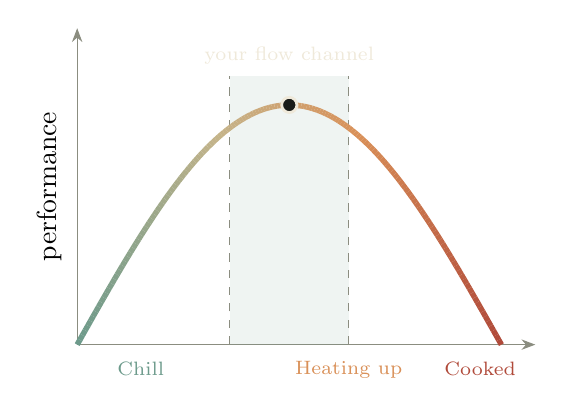
\begin{tikzpicture}
        \begin{axis}[
          darkpanel,
          width=7.4cm, height=5.6cm,
          clip=false,
          axis line style={-{Stealth[length=5pt]}, InkFaint},
          xmin=0, xmax=10.8, ymin=0, ymax=1.32,
          xtick=\empty, ytick=\empty,
          ylabel={performance},
          colormap={flow}{color=(Sage) color=(Tan) color=(Amber) color=(Rust)},
        ]
          % flow-channel band
          \fill[Sage, opacity=0.11]
            (axis cs:3.6,0) rectangle (axis cs:6.4,1.12);
          \draw[InkFaint, dashed] (axis cs:3.6,0) -- (axis cs:3.6,1.12);
          \draw[InkFaint, dashed] (axis cs:6.4,0) -- (axis cs:6.4,1.12);
          \node[font=\scriptsize, color=Ink, anchor=south]
            at (axis cs:5,1.13) {your flow channel};
          % gradient arc (Chill -> Cooked)
          \addplot[
            mesh, shader=flat, point meta=x,
            line width=2pt, samples=160, domain=0:10, forget plot,
          ] {sin(x*18)};
          % operating-point marker at the peak
          \node[circle, draw=Ink, line width=1pt, fill=SlideBg,
                inner sep=0, minimum size=5.5pt] at (axis cs:5,1.0) {};
          % zone labels
          \node[font=\scriptsize, color=Sage, anchor=north]
            at (axis cs:1.5,-0.03) {Chill};
          \node[font=\scriptsize, color=Amber, anchor=north]
            at (axis cs:6.4,-0.03) {Heating up};
          \node[font=\scriptsize, color=Rust, anchor=north]
            at (axis cs:9.5,-0.03) {Cooked};
        \end{axis}
      \end{tikzpicture}%
      }
    \end{column}
  \end{columns}
\end{frame}

% =========================================================================
\section{The problem}
% =========================================================================

% F2 · The role has shifted
\begin{frame}{Software engineers stopped typing most of their code}
  \begin{columns}[T]
    \begin{column}{0.56\textwidth}
      \begin{itemize}
        \item Coding agents produce code at machine pace, in
              \good{concurrent sessions}.
        \item The human role becomes \good{supervision}: dispatch tasks,
              monitor progress, judge partial results, re-engage failed or
              dormant threads.
        \item The natural incentive (\warnc{``tokenmaxxing''}) is to run as
              many sessions as possible: tokens are cheap, attention is not.
        \item The binding resource is no longer typing speed. It is
              \alert{one person's attention}.
      \end{itemize}
      \vfill
      \src{Sheridan (1992), \emph{Telerobotics, Automation, and Human
      Supervisory Control}: the operator who time-shares across
      semi-autonomous processes.}
    \end{column}
    \begin{column}{0.40\textwidth}
      \centering
      \resizebox{0.88\linewidth}{!}{%
      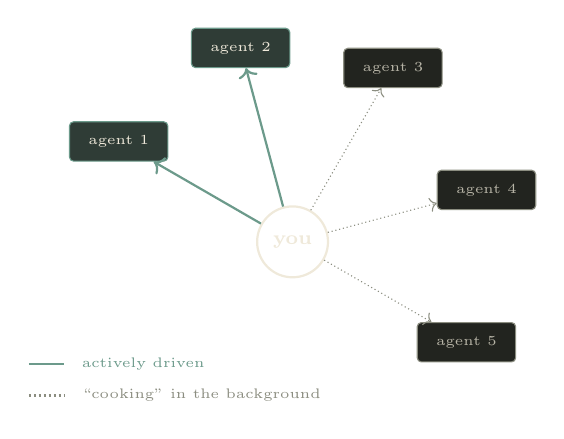
\begin{tikzpicture}[x=1cm,y=1cm]
        \node[circle,draw=Ink,thick,minimum size=9mm,text=Ink,
              font=\scriptsize\bfseries] (op) at (0,0) {you};
        \foreach \ang/\w/\lab in {150/1/{agent 1}, 105/1/{agent 2},
                                  60/0/{agent 3}, 15/0/{agent 4},
                                  -30/0/{agent 5}} {
          \ifnum\w=1
            \node[draw=Sage,fill=Sage!25!SlideBg,rounded corners=1.5pt,
                  text=Ink,font=\tiny,minimum width=12.5mm,minimum height=5mm]
                  (a\ang) at (\ang:2.55) {\lab};
            \draw[->,Sage,thick] (op) -- (a\ang);
          \else
            \node[draw=InkFaint,fill=Panel,rounded corners=1.5pt,
                  text=InkSoft,font=\tiny,minimum width=12.5mm,minimum height=5mm]
                  (a\ang) at (\ang:2.55) {\lab};
            \draw[->,InkFaint,densely dotted] (op) -- (a\ang);
          \fi
        }
        \draw[Sage,thick] (-3.35,-1.55) -- (-2.90,-1.55);
        \node[font=\tiny,text=Sage,anchor=west] at (-2.80,-1.55)
              {actively driven};
        \draw[InkFaint,densely dotted,thick] (-3.35,-1.95) -- (-2.90,-1.95);
        \node[font=\tiny,text=InkFaint,anchor=west] at (-2.80,-1.95)
              {``cooking'' in the background};
      \end{tikzpicture}%
      }
    \end{column}
  \end{columns}
\end{frame}

% F3 · Other professions got there first
\begin{frame}{Other professions got there first}
  \small Automation does not subtract work. It converts
  \good{producers} into \warnc{supervisors of parallel output}, and the
  residual monitoring role gets harder, not easier.\par
  \src{Bainbridge (1983), ``Ironies of Automation.''}
  \vspace{1.5mm}
  \begin{tabular}{@{}p{0.185\textwidth}p{0.72\textwidth}@{}}
    \good{Aviation} & Cockpit automation moved pilots from flying to
      monitoring: vigilance decrement, ``automation surprises.''
      \soft{Wiener \& Curry (1980)} \\[2.5pt]
    \good{Anesthesiology} & One anesthesiologist directs several operating
      rooms at once; higher ratios are associated with worse patient
      outcomes. \soft{Burns et al.\ (2022)} \\[2.5pt]
    \good{Air traffic} & Controller workload scales with the number of
      aircraft held; decision support exists precisely to raise that count.
      \soft{Loft et al.\ (2007)} \\[2.5pt]
    \good{Radiology} & Cross-sectional imaging multiplied images per study;
      an image to interpret every few seconds across a shift.
      \soft{McDonald et al.\ (2015)} \\[2.5pt]
    \good{Translation} & Post-editing machine output turns translators into
      high-throughput reviewers; the result is measurably flatter.
      \soft{Krings (2001); Toral (2019)}
  \end{tabular}\par
\end{frame}

% F4 · What supervisory control already knows
\begin{frame}{What supervisory-control research already knows}
  \begin{itemize}
    \item \good{Fan-out}: how many semi-autonomous units one operator can
          manage, bounded by \emph{neglect time} and \emph{interaction time}.
          \src{Crandall \& Cummings (2007); Cummings \& Mitchell (2008), for UAV/robot operators.}
    \item Past a personal fan-out limit, performance collapses
          \alert{non-linearly}, often \alert{before the operator notices}.
          \src{Cummings \& Mitchell (2008).}
    \item Staying out of the loop degrades situation awareness and taxes
          re-engagement. \src{Endsley \& Kiris (1995); Eriksson \& Stanton (2017).}
    \item Monitoring an autonomous process is not idle time: it is
          \warnc{effortful and stress-inducing}. \src{Warm, Parasuraman \& Matthews (2008).}
    \item Under concurrent load, operators systematically under-monitor:
          \warnc{complacency}. \src{Parasuraman \& Manzey (2010).}
  \end{itemize}
  \vspace{1mm}
  {\small Supervising LLM coding agents is the \good{same control problem}
   in a new domain; the transfer is plausible, and testing it is part of
   this work.\par}
\end{frame}

% F5 · Effort shifts, not disappears
\begin{frame}{In software, the effort shifts rather than disappears}
  \begin{itemize}
    \item Software engineers spend \good{$\approx$51.5\% of session time} in
          assistant-specific states: verifying suggestions, prompt-crafting,
          deferring thought.
          \src{Mozannar, Bansal, Fourney \& Horvitz (2024), CHI.}
    \item Merely \emph{informing} engineers that code is LLM-generated
          raises their measured NASA-TLX workload.
          \src{Tang et al.\ (2024), IEEE VL/HCC.}
    \item The interaction is bimodal: fast \emph{acceleration} alternating
          with slow, validation-heavy \emph{exploration}.
          \src{Barke, James \& Polikarpova (2023).}
    \item A mixed-methods survey of 442 software engineers links GenAI
          adoption to \warnc{burnout through intensified job demands}.
          \src{Feng, Afroz \& Sarma (2026), ICSE-SEIS; Demerouti et al.\ (2001), Job Demands--Resources.}
  \end{itemize}
\end{frame}

% F6 · Oversight degrades quietly
\begin{frame}{And oversight quality degrades quietly}
  \begin{itemize}
    \item With an AI assistant, users wrote \badc{less secure code} while
          being \badc{more confident} it was secure.
          \src{Perry, Srivastava, Kumar \& Boneh (2023), ACM CCS.}
    \item Professional engineers show automation complacency and rising
          reliance over the course of a single task.
          \src{Qian \& Wexler (2024), ACM IUI.}
    \item In human code inspection, defect-removal effectiveness
          \alert{falls sharply past $\approx$200 lines reviewed per hour};
          review rate is the dominant controllable factor.
          \src{Kemerer \& Paulk (2009); the general speed--accuracy trade-off, Wickelgren (1977).}
  \end{itemize}
  \vspace{1mm}
  {\small More parallel output funneled into the same reviewing hours means
   \alert{each change gets less scrutiny} --- reviewers are forced to go
   faster, compounding the complacency findings above.\par}
\end{frame}

% F7 · Invisible from the inside
\begin{frame}{The load is invisible from the inside}
  \begin{columns}[T]
    \begin{column}{0.56\textwidth}
      \begin{itemize}
        \item Randomized trial: experienced open-source developers were
              \badc{$\approx$19\% slower} with AI tooling, yet
              \badc{believed it sped them up}.
              \src{Becker, Rush, Barnes \& Rein (2025), METR; preprint.}
        \item The perception--reality gap recurs in longitudinal IDE
              telemetry and in a 49{,}000-respondent survey.
              \src{Sergeyuk et al.\ (2026), ICSE; Stack Overflow (2025).}
        \item If a marginal session consumes attention faster than it yields
              verified output, adding sessions is
              \alert{counterproductive}.
      \end{itemize}
    \end{column}
    \begin{column}{0.42\textwidth}
      \centering
      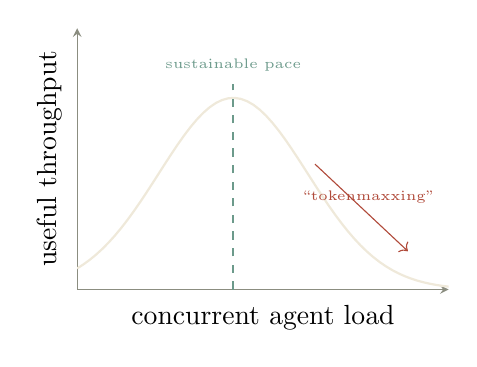
\begin{tikzpicture}
        \begin{axis}[darkpanel, width=6.3cm, height=4.9cm,
            xlabel={concurrent agent load},
            ylabel={useful throughput},
            xmin=0, xmax=10, ymin=0, ymax=1.5,
            xtick=\empty, ytick=\empty]
          \addplot[Ink, thick, domain=0:10, samples=60]
            {1.1*exp(-((x-4.2)^2)/8)};
          \draw[dashed, Sage, thick] (axis cs:4.2,0) -- (axis cs:4.2,1.18);
          \node[font=\tiny, color=Sage, anchor=south] at (axis cs:4.2,1.20)
            {sustainable pace};
          \draw[->, Rust] (axis cs:6.4,0.72) -- (axis cs:8.9,0.22);
          \node[font=\tiny, color=Rust, anchor=north east] at (axis cs:9.9,0.62)
            {``tokenmaxxing''};
        \end{axis}
      \end{tikzpicture}
      \src{Inverted-U of performance under load: Yerkes \& Dodson (1908);
           the flow channel, Csikszentmihalyi (1990).}
    \end{column}
  \end{columns}
\end{frame}

% F8 · Problem statement
\begin{frame}{The problem, stated}
  \begin{itemize}
    \item Kanban caps work-in-progress \emph{not to slow delivery} but to
          protect flow and a sustainable pace.
          \src{Anderson (2010); Beck (2000).}
    \item Concurrent agent supervision is the same control problem with the
          WIP limit relocated \alert{into one human's working memory},
          where it is ordinarily invisible.
    \item The aim is \good{not} to use agents less: it is to find each
          person's operating band where throughput and supervision quality
          are jointly sustained.
  \end{itemize}
  \vspace{2mm}
  \begin{beamercolorbox}[rounded=true,sep=6pt]{block body}
    \small What is missing is the \good{signal}: a private,
    longitudinal, research-grounded view of one's own supervision load,
    scored against one's \emph{own} history, with a personally discovered
    optimum to steer toward.
  \end{beamercolorbox}
\end{frame}

% =========================================================================
\section{The instrument}
% =========================================================================

% F9 · Pipeline
\begin{frame}{From logs already on disk to a daily score}
  \centering
  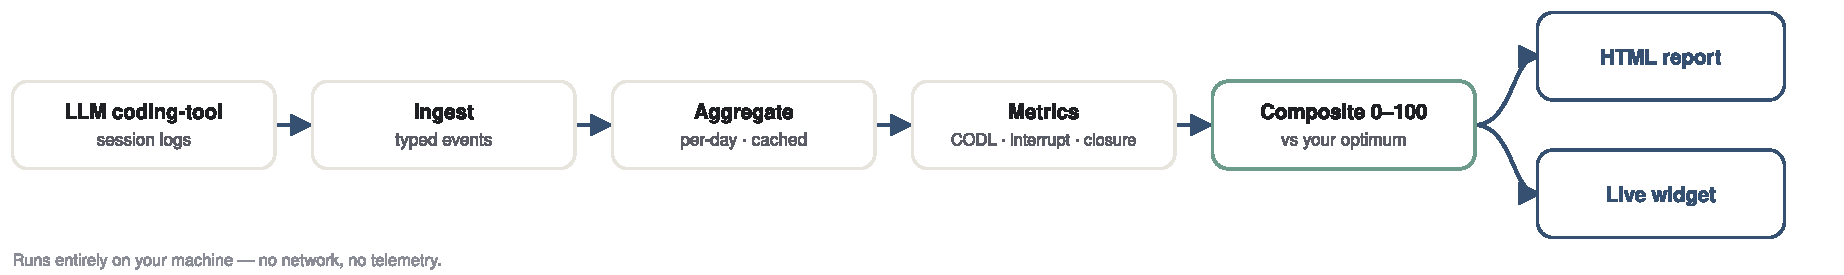
\includegraphics[width=0.97\textwidth]{pipeline.pdf}
  \vspace{2mm}
  \begin{itemize}
    \item Input: the session logs agent-coding tools \good{already write
          locally} (Claude Code, Codex CLI, \ldots); one small adapter per
          tool maps them to typed events.
    \item Per-day aggregation with caching; three axes; a composite scored
          against a personal baseline and optimum.
    \item Python standard library only; \good{no network I/O at any stage};
          output is a self-contained HTML report plus a JSON sibling.
  \end{itemize}
\end{frame}

% F10 · CODL
\begin{frame}{Axis 1 $\cdot$ CODL: engagement-weighted concurrency}
  \begin{columns}[T]
    \begin{column}{0.60\textwidth}
      \centering
      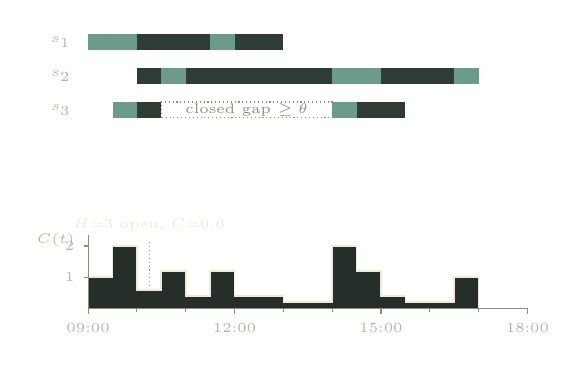
\begin{tikzpicture}[x=0.62cm, y=0.72cm]
        % stream rows
        \node[anchor=east, font=\tiny, text=InkSoft] at (-0.15,4.70) {$s_1$};
        \fill[Sage]              (0,4.56)   rectangle (1,4.84);
        \fill[Sage!25!SlideBg]   (1,4.56)   rectangle (2.5,4.84);
        \fill[Sage]              (2.5,4.56) rectangle (3,4.84);
        \fill[Sage!25!SlideBg]   (3,4.56)   rectangle (4,4.84);
        \node[anchor=east, font=\tiny, text=InkSoft] at (-0.15,4.10) {$s_2$};
        \fill[Sage!25!SlideBg]   (1,3.96)   rectangle (1.5,4.24);
        \fill[Sage]              (1.5,3.96) rectangle (2,4.24);
        \fill[Sage!25!SlideBg]   (2,3.96)   rectangle (5,4.24);
        \fill[Sage]              (5,3.96)   rectangle (6,4.24);
        \fill[Sage!25!SlideBg]   (6,3.96)   rectangle (7.5,4.24);
        \fill[Sage]              (7.5,3.96) rectangle (8,4.24);
        \node[anchor=east, font=\tiny, text=InkSoft] at (-0.15,3.50) {$s_3$};
        \fill[Sage]              (0.5,3.36) rectangle (1,3.64);
        \fill[Sage!25!SlideBg]   (1,3.36)   rectangle (1.5,3.64);
        \draw[densely dotted, InkFaint] (1.5,3.36) rectangle (5,3.64);
        \node[font=\tiny, text=InkFaint] at (3.25,3.50) {closed gap $\ge\theta$};
        \fill[Sage]              (5,3.36)   rectangle (5.5,3.64);
        \fill[Sage!25!SlideBg]   (5.5,3.36) rectangle (6.5,3.64);
        % C(t)
        \begin{scope}[yscale=0.55]
        \fill[Sage!14!SlideBg]
          (0,0) -- (0,1.0) -- (0.5,1.0) -- (0.5,2.0) -- (1,2.0) -- (1,0.6)
          -- (1.5,0.6) -- (1.5,1.2) -- (2,1.2) -- (2,0.4) -- (2.5,0.4)
          -- (2.5,1.2) -- (3,1.2) -- (3,0.4) -- (4,0.4) -- (4,0.2) -- (5,0.2)
          -- (5,2.0) -- (5.5,2.0) -- (5.5,1.2) -- (6,1.2) -- (6,0.4)
          -- (6.5,0.4) -- (6.5,0.2) -- (7.5,0.2) -- (7.5,1.0) -- (8,1.0)
          -- (8,0) -- cycle;
        \draw[Ink, semithick]
          (0,1.0) -- (0.5,1.0) -- (0.5,2.0) -- (1,2.0) -- (1,0.6) -- (1.5,0.6)
          -- (1.5,1.2) -- (2,1.2) -- (2,0.4) -- (2.5,0.4) -- (2.5,1.2)
          -- (3,1.2) -- (3,0.4) -- (4,0.4) -- (4,0.2) -- (5,0.2) -- (5,2.0)
          -- (5.5,2.0) -- (5.5,1.2) -- (6,1.2) -- (6,0.4) -- (6.5,0.4)
          -- (6.5,0.2) -- (7.5,0.2) -- (7.5,1.0) -- (8,1.0) -- (8,0) -- (9,0);
        \draw[InkFaint] (0,0) -- (0,2.35);
        \foreach \c in {1,2} {\draw[InkFaint] (-0.08,\c) -- (0,\c);
          \node[anchor=east, font=\tiny, text=InkSoft] at (-0.08,\c) {$\c$};}
        \node[anchor=east, font=\tiny, text=InkSoft] at (-0.08,2.2) {$C(t)$};
        \node[anchor=south, font=\tiny, text=Ink] at (1.25,2.15)
          {$H{=}3$ open, $C{=}0.6$};
        \draw[densely dotted, InkFaint] (1.25,2.12) -- (1.25,0.66);
        \end{scope}
        \draw[InkFaint] (0,0) -- (9,0);
        \foreach \x in {1,2,4,5,7,8} \draw[InkFaint] (\x,0) -- (\x,-0.06);
        \foreach \x/\l in {0/09:00, 3/12:00, 6/15:00, 9/18:00}
          {\draw[InkFaint] (\x,0) -- (\x,-0.10);
           \node[anchor=north, font=\tiny, text=InkSoft] at (\x,-0.10) {\l};}
      \end{tikzpicture}
    \end{column}
    \begin{column}{0.38\textwidth}
      \small
      \begin{itemize}
        \item A session is \good{foreground} ($e_s{=}1$) within $g{=}5$\,min
              of \emph{your own} message.
        \item Otherwise, while live, it \warnc{``cooks''} at weight
              $\beta{=}0.2$; a closed tool counts \soft{nothing}.
        \item Weighted concurrency $C(t)$ is charged per minute against
              working-memory capacity $\kappa\approx4$, accumulating a
              \good{capacity-dose} toward a 240-min horizon.
      \end{itemize}
      \src{Working memory holds $\approx$4 independent items:
           Cowan (2001). Fan-out and attention demand:
           Crandall \& Cummings (2007).}
    \end{column}
  \end{columns}
\end{frame}

% F11 · Beta grounding
\begin{frame}{Background sessions are not free: the case for $\beta > 0$}
  \begin{itemize}
    \item A session left running while attention is elsewhere is the
          \good{out-of-the-loop regime} of supervisory control, not rest.
    \item Monitoring is \warnc{effortful and stressful} even when nothing is
          wrong. \src{Warm, Parasuraman \& Matthews (2008).}
    \item Re-engaging costs: situation awareness decays out of the loop.
          \src{Endsley \& Kiris (1995); Eriksson \& Stanton (2017).}
    \item Under load, monitoring quietly degrades: \warnc{complacency}.
          \src{Parasuraman \& Manzey (2010).}
    \item Magnitude borrowed from prospective memory: holding a pending
          intention slows the ongoing task by \good{15--20\%}, and open
          goals occupy memory until closed or planned.
          \src{Smith (2003); Masicampo \& Baumeister (2011).}
  \end{itemize}
  \vspace{1mm}
  {\small Hence $\beta=0.20$, the top of that band: a \good{defensible,
   auditable prior}, exposed in configuration rather than hard-coded, and a
   named target for calibration.\par}
\end{frame}

% F12 · Interruption Index
\begin{frame}{Axis 2 $\cdot$ Interruption Index}
  \begin{itemize}
    \item Counts the events that \alert{pull attention}: tool
          \warnc{errors} (weight 1.5) and \warnc{cross-stream starts}
          (weight 3.0), per work hour.
    \item Routine tool calls are \good{deliberately not counted}: while an
          agent works, the operator is legitimately waiting, and counting
          each call would inflate the rate by orders of magnitude.
    \item Normalization ceiling 10/hour, above the knowledge-work baseline
          of a working-sphere switch about every 11 minutes
          ($\approx$5/hour).
          \src{Gonz\'alez \& Mark (2004), CHI.}
    \item Why it matters: interrupted work completes \emph{faster} but at
          higher stress and effort; unfinished-task residue impairs the next
          task; cross-tool switches cost more than within-tool ones.
          \src{Mark, Gudith \& Klocke (2008); Mark, Gonzalez \& Harris (2005);
               Leroy (2009); Wickens (2008).}
  \end{itemize}
\end{frame}

% F13 · Closure Deficit
\begin{frame}{Axis 3 $\cdot$ Closure Deficit: the cost of coming back}
  \begin{columns}[T]
    \begin{column}{0.47\textwidth}
      \centering
      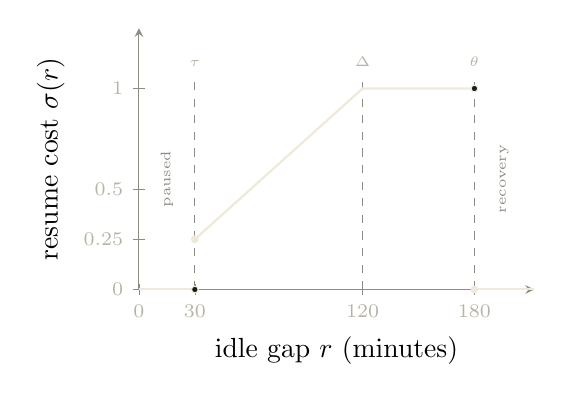
\begin{tikzpicture}
        \begin{axis}[darkpanel, width=6.6cm, height=4.9cm,
          xlabel={idle gap $r$ (minutes)}, ylabel={resume cost $\sigma(r)$},
          xmin=0, xmax=212, ymin=0, ymax=1.3,
          xtick={0,30,120,180}, ytick={0,0.25,0.5,1}]
          \draw[dashed, InkFaint] (axis cs:30,0) -- (axis cs:30,1.06);
          \draw[dashed, InkFaint] (axis cs:120,0) -- (axis cs:120,1.06);
          \draw[dashed, InkFaint] (axis cs:180,0) -- (axis cs:180,1.06);
          \node[anchor=south, font=\tiny, color=InkSoft] at (axis cs:30,1.06) {$\tau$};
          \node[anchor=south, font=\tiny, color=InkSoft] at (axis cs:120,1.06) {$\Delta$};
          \node[anchor=south, font=\tiny, color=InkSoft] at (axis cs:180,1.06) {$\theta$};
          \node[color=InkFaint, rotate=90, font=\tiny] at (axis cs:15,0.55) {paused};
          \node[color=InkFaint, rotate=90, font=\tiny] at (axis cs:196,0.55) {recovery};
          \addplot[Ink, thick] coordinates {(0,0) (30,0)};
          \addplot[Ink, thick] coordinates {(30,0.25) (120,1) (180,1)};
          \addplot[Ink, thick] coordinates {(180,0) (212,0)};
          \addplot[only marks, mark=*, mark size=1.2, Ink]
            coordinates {(30,0.25) (180,0)};
          \addplot[only marks, mark=*, mark size=1.2, Ink,
                   mark options={fill=SlideBg}]
            coordinates {(30,0) (180,1)};
        \end{axis}
      \end{tikzpicture}
    \end{column}
    \begin{column}{0.51\textwidth}
      \small
      \begin{itemize}
        \item A \good{resume} is a true-idle gap in one session, picked back
              up later: below $\tau{=}30$\,min it was merely paused; at
              $\theta{=}3$\,h the break counts as recovery, a fresh sitting.
        \item Cost saturates at $\Delta{=}120$\,min: the context has gone
              \warnc{fully cold}. Daily ceiling: about
              \good{4 cold reloads}.
      \end{itemize}
      \src{Suspended goals decay and must be reconstructed:
           Altmann \& Trafton (2002). Resumption lag grows with
           interruption duration: Monk, Trafton \& Boehm-Davis (2008).
           Interrupted programmers rarely resume coding within a minute:
           Parnin \& Rugaber (2011). Closure as a recovery resource:
           Sonnentag \& Fritz (2007).}
    \end{column}
  \end{columns}
\end{frame}

% F14 · Composite + off-hours
\begin{frame}{Composite score}
  \begin{columns}[T]
    \begin{column}{0.55\textwidth}
      \small
      \begin{itemize}
        \item Composite $=$ equal-weight mean of the three axes, on
              0--100. Equal weights are the \good{explicit null
              hypothesis}, not a finding; calibrating them is named future
              work.
        \item Engaged minutes \emph{outside your own inferred hours} add an
              additive toll: up to \warnc{$+30$ points}, saturating at
              90 minutes.
        \item The boundary is asymmetric: evenings count in full, an early
              start gets a grace. The recovery literature locates the harm
              in \alert{failure to disengage at day's end}.
              \src{Sonnentag \& Fritz (2007); Sonnentag, Binnewies \& Mojza (2010);
                   sustained activation, not peaks: McEwen (1998).}
        \item Every day is colored against \good{your own} p50/p75/p90,
              never a population norm.
      \end{itemize}
    \end{column}
    \begin{column}{0.42\textwidth}
      \centering
      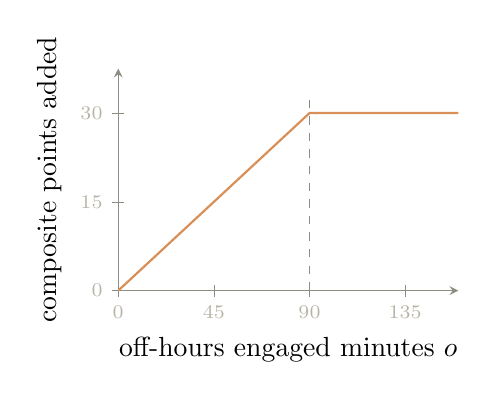
\begin{tikzpicture}
        \begin{axis}[darkpanel, width=5.9cm, height=4.4cm,
          xlabel={off-hours engaged minutes $o$},
          ylabel={composite points added},
          xmin=0, xmax=160, ymin=0, ymax=37.5,
          xtick={0,45,90,135}, ytick={0,15,30}]
          \draw[dashed, InkFaint] (axis cs:90,0) -- (axis cs:90,33);
          \addplot[Amber, thick] coordinates {(0,0) (90,30) (160,30)};
        \end{axis}
      \end{tikzpicture}
      \src{Anchored to interaction: a background session running while
           you are away adds nothing; only engaged off-hours minutes count.}
    \end{column}
  \end{columns}
\end{frame}

% F15 · Personal optimum
\begin{frame}{Personal optimum}
  \begin{columns}[T]
    \begin{column}{0.52\textwidth}
      \centering
      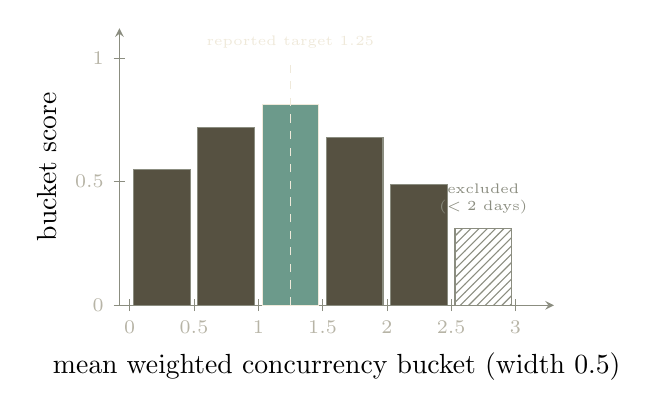
\begin{tikzpicture}
        \begin{axis}[darkpanel, width=7.1cm, height=5.1cm,
          xlabel={mean weighted concurrency bucket (width $0.5$)},
          ylabel={bucket score},
          xmin=-0.08, xmax=3.3, ymin=0, ymax=1.12,
          xtick={0,0.5,1,1.5,2,2.5,3}, ytick={0,0.5,1}]
          \fill[Tan!35!SlideBg, draw=InkFaint] (axis cs:0.03,0) rectangle (axis cs:0.47,0.55);
          \fill[Tan!35!SlideBg, draw=InkFaint] (axis cs:0.53,0) rectangle (axis cs:0.97,0.72);
          \fill[Sage, draw=Ink]                (axis cs:1.03,0) rectangle (axis cs:1.47,0.81);
          \fill[Tan!35!SlideBg, draw=InkFaint] (axis cs:1.53,0) rectangle (axis cs:1.97,0.68);
          \fill[Tan!35!SlideBg, draw=InkFaint] (axis cs:2.03,0) rectangle (axis cs:2.47,0.49);
          \fill[pattern=north east lines, pattern color=InkFaint, draw=InkFaint]
            (axis cs:2.53,0) rectangle (axis cs:2.97,0.31);
          \node[anchor=south, align=center, font=\tiny, color=InkFaint]
            at (axis cs:2.75,0.33) {excluded\\($<2$ days)};
          \draw[dashed, Ink] (axis cs:1.25,0) -- (axis cs:1.25,1.0);
          \node[anchor=south, font=\tiny, color=Ink] at (axis cs:1.25,1.0)
            {reported target $1.25$};
        \end{axis}
      \end{tikzpicture}
    \end{column}
    \begin{column}{0.46\textwidth}
      \small
      \begin{itemize}
        \item Historical days are bucketed by mean weighted concurrency;
              each bucket is rewarded for \good{closing loops} and
              penalised for \warnc{spilling past the window}.
        \item The best bucket's midpoint becomes the
              \good{flow-channel target}: a line to steer toward, not a
              ceiling to stay under.
        \item This is a personal work-in-progress limit made
              \emph{discoverable from one's own data}; it needs 14 active
              days, and shows ``calibrating'' before that.
      \end{itemize}
      \src{Inverted-U of performance under load: Yerkes \& Dodson (1908).
           The flow channel between boredom and anxiety:
           Csikszentmihalyi (1990).}
    \end{column}
  \end{columns}
\end{frame}

% =========================================================================
\section{The tool}
% =========================================================================

% F16 · Year report
\begin{frame}{A year against your own baseline}
  \begin{columns}[T]
    \begin{column}{0.63\textwidth}
      \centering
      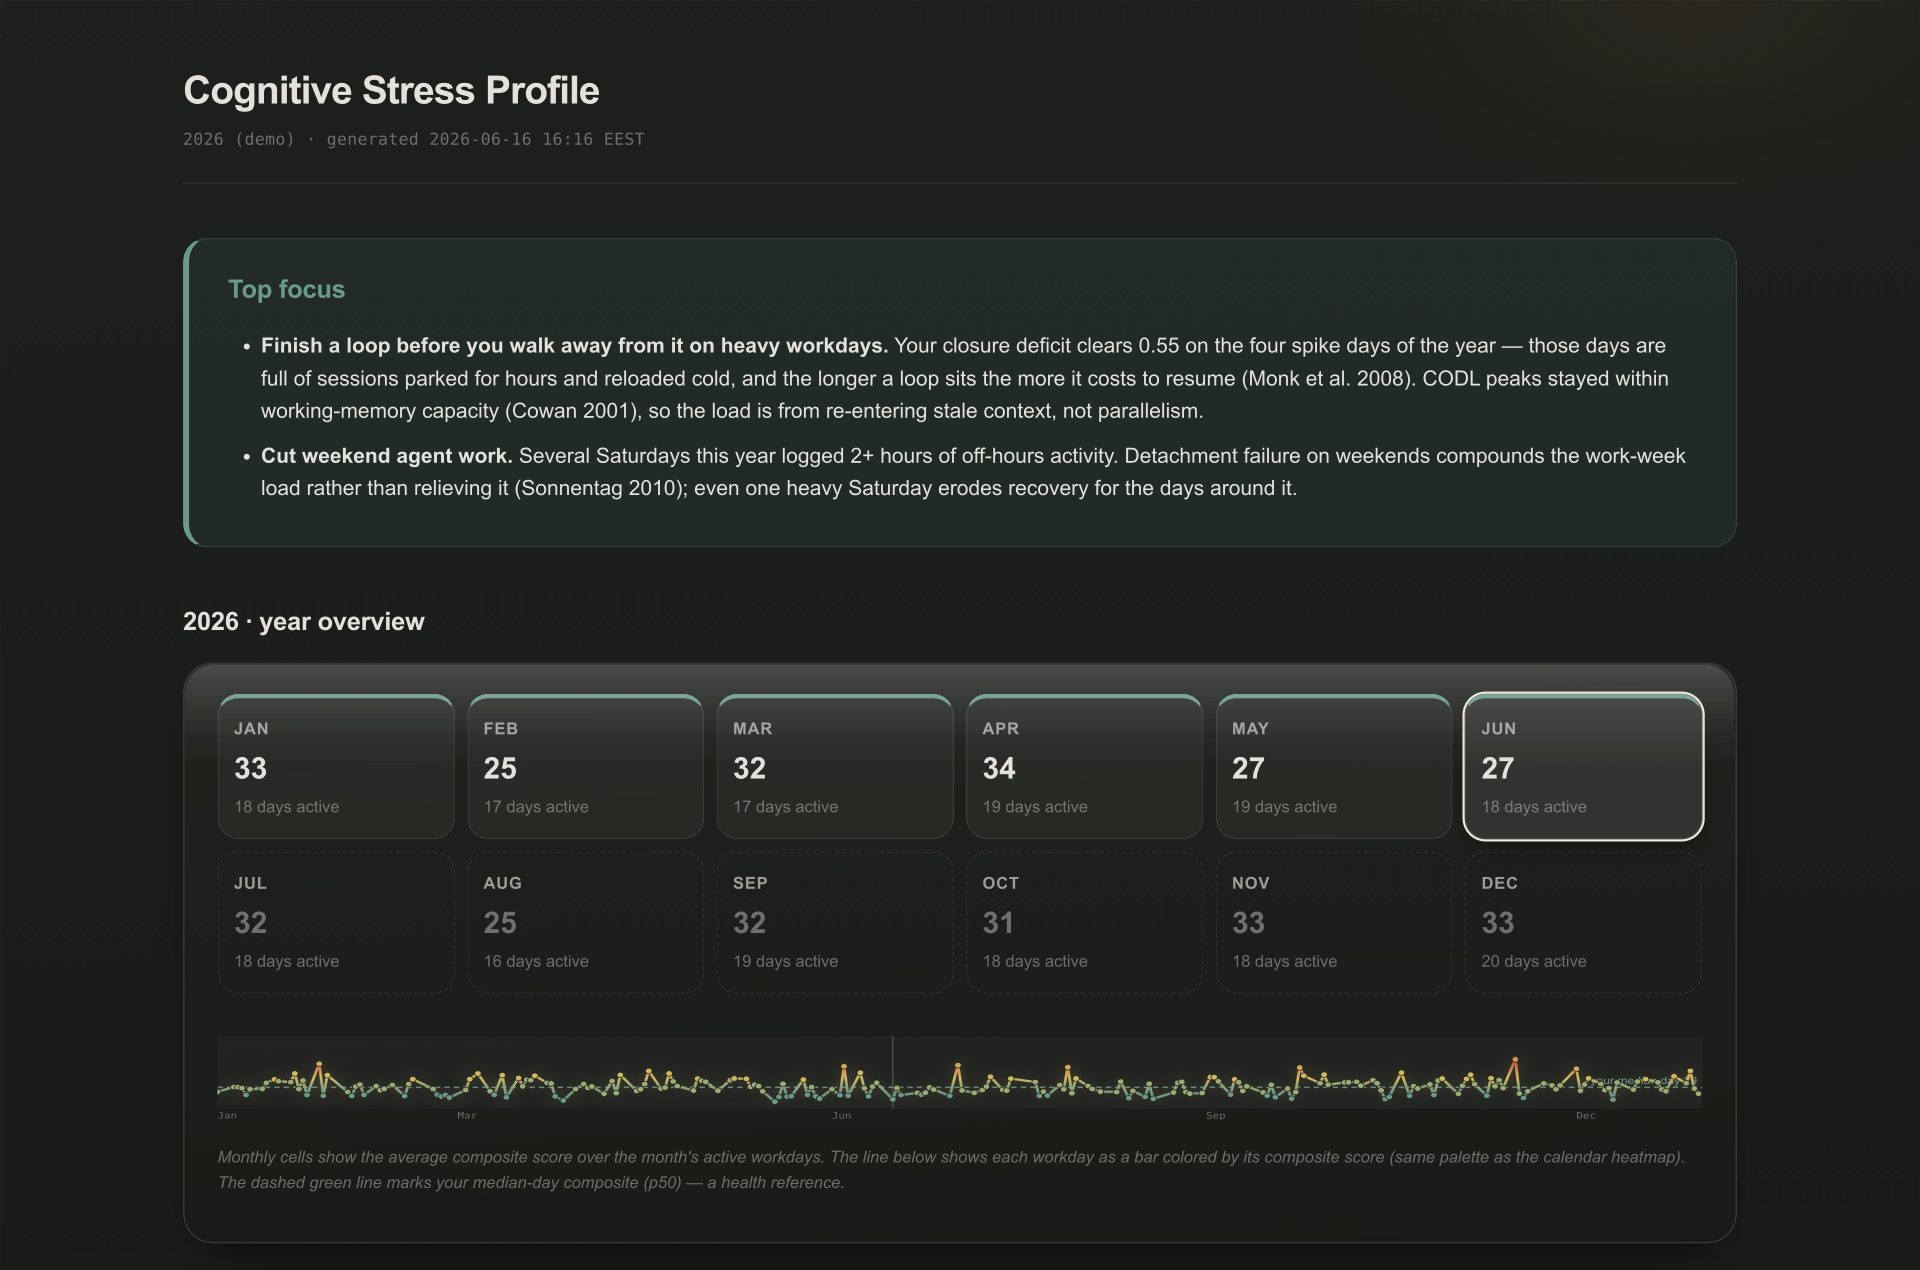
\includegraphics[width=\textwidth]{overview-top.png}
    \end{column}
    \begin{column}{0.35\textwidth}
      \small
      \begin{itemize}
        \item One self-contained HTML file; a JSON sibling for scripts and
              chat skills.
        \item Twelve monthly cells with active-day counts, plus a
              day-by-day strip against the personal median.
        \item ``Top focus'' guidance up front, each recommendation tied to
              the literature behind it.
      \end{itemize}
      \src{Shown throughout: the tool's deterministic synthetic
           demonstration dataset; no operator's activity is exposed.}
    \end{column}
  \end{columns}
\end{frame}

% F17 · Month view
\begin{frame}{Months as calendars, days against percentiles}
  \begin{columns}[T]
    \begin{column}{0.63\textwidth}
      \centering
      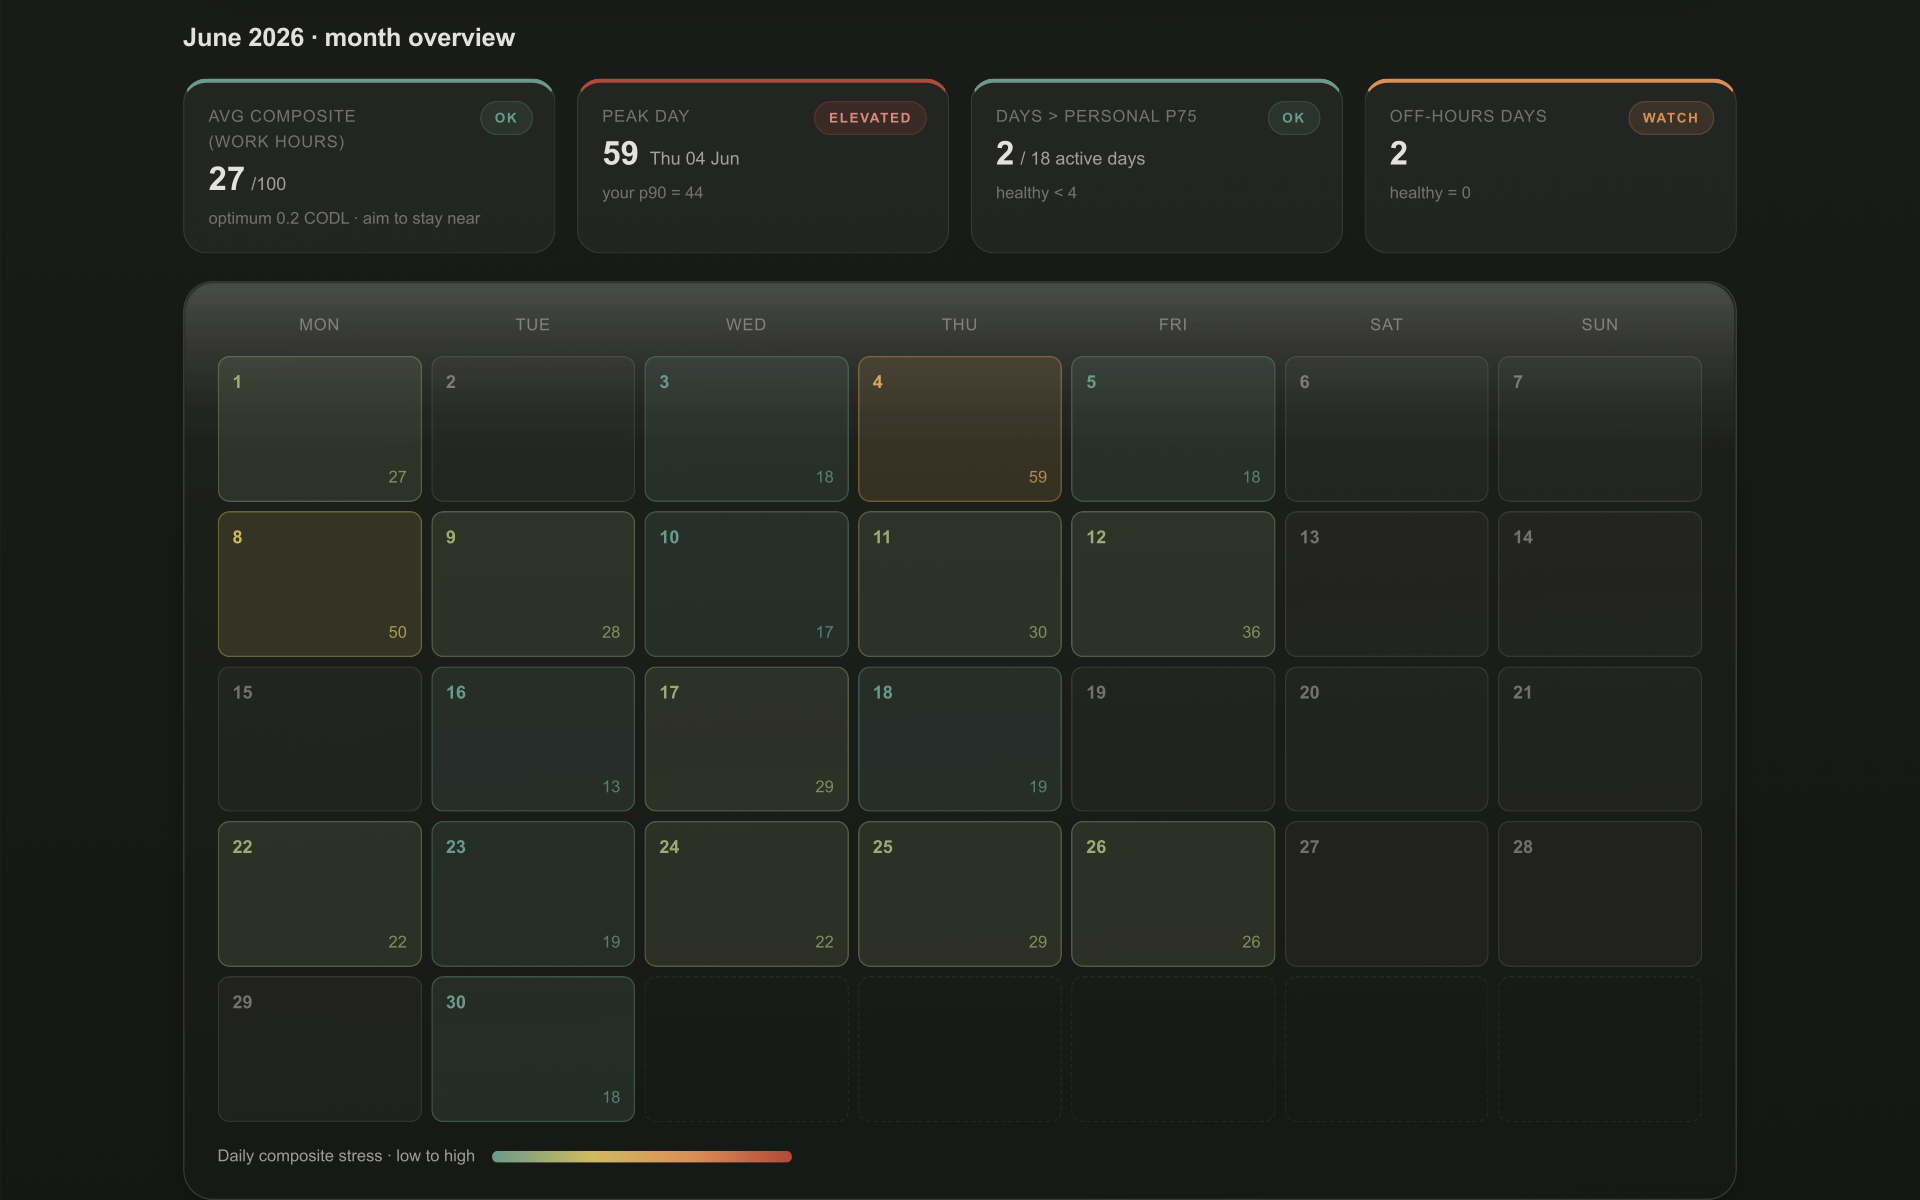
\includegraphics[width=\textwidth]{overview-month.png}
    \end{column}
    \begin{column}{0.35\textwidth}
      \small
      \begin{itemize}
        \item KPI tiles: average composite against the personal optimum,
              peak day, days above the personal p75, off-hours days.
        \item Calendar heatmap colored by each day's composite,
              \good{relative to your own history}.
        \item Zones use the same scale everywhere: report, JSON, and
              widgets can never drift apart.
      \end{itemize}
    \end{column}
  \end{columns}
\end{frame}

% F18 · Day drill-down
\begin{frame}{Any day, drilled down}
  \begin{columns}[T]
    \begin{column}{0.60\textwidth}
      \centering
      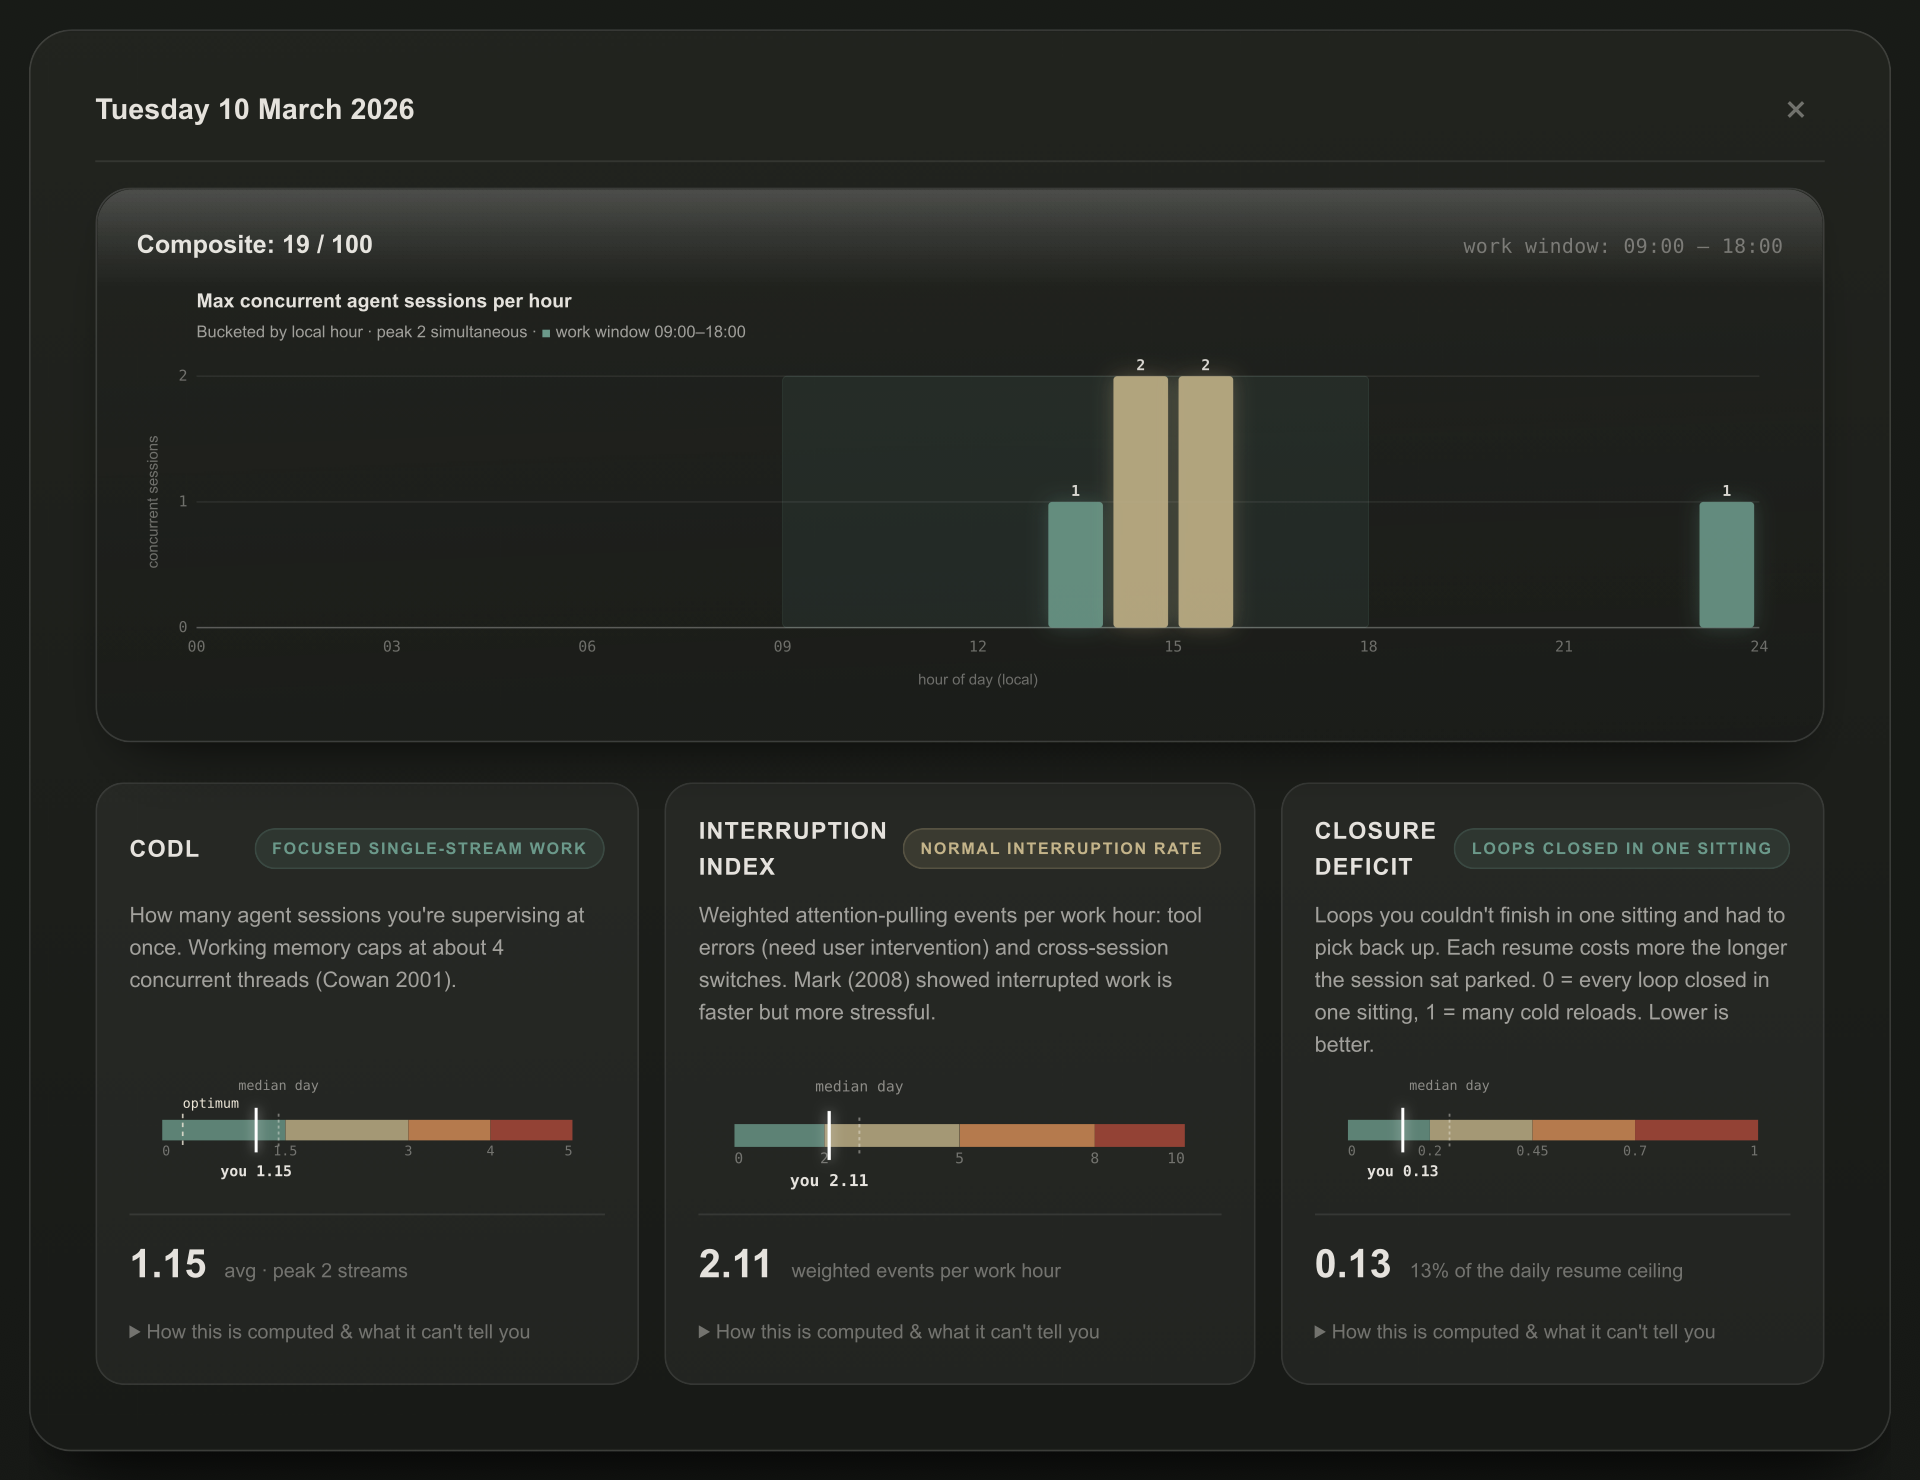
\includegraphics[width=\textwidth]{day-modal.png}
    \end{column}
    \begin{column}{0.38\textwidth}
      \small
      \begin{itemize}
        \item Hourly concurrency inside the inferred work window.
        \item The three axes as tiles, each placed on its zone scale
              against a \good{typical day} marker.
        \item Every tile explains \emph{how it is computed and what it
              cannot tell you}: the limitations ship inside the report.
      \end{itemize}
    \end{column}
  \end{columns}
\end{frame}

% F19 · Widgets
\begin{frame}{Ambient, glanceable, always on}
  \begin{columns}[T]
    \begin{column}{0.60\textwidth}
      \centering
      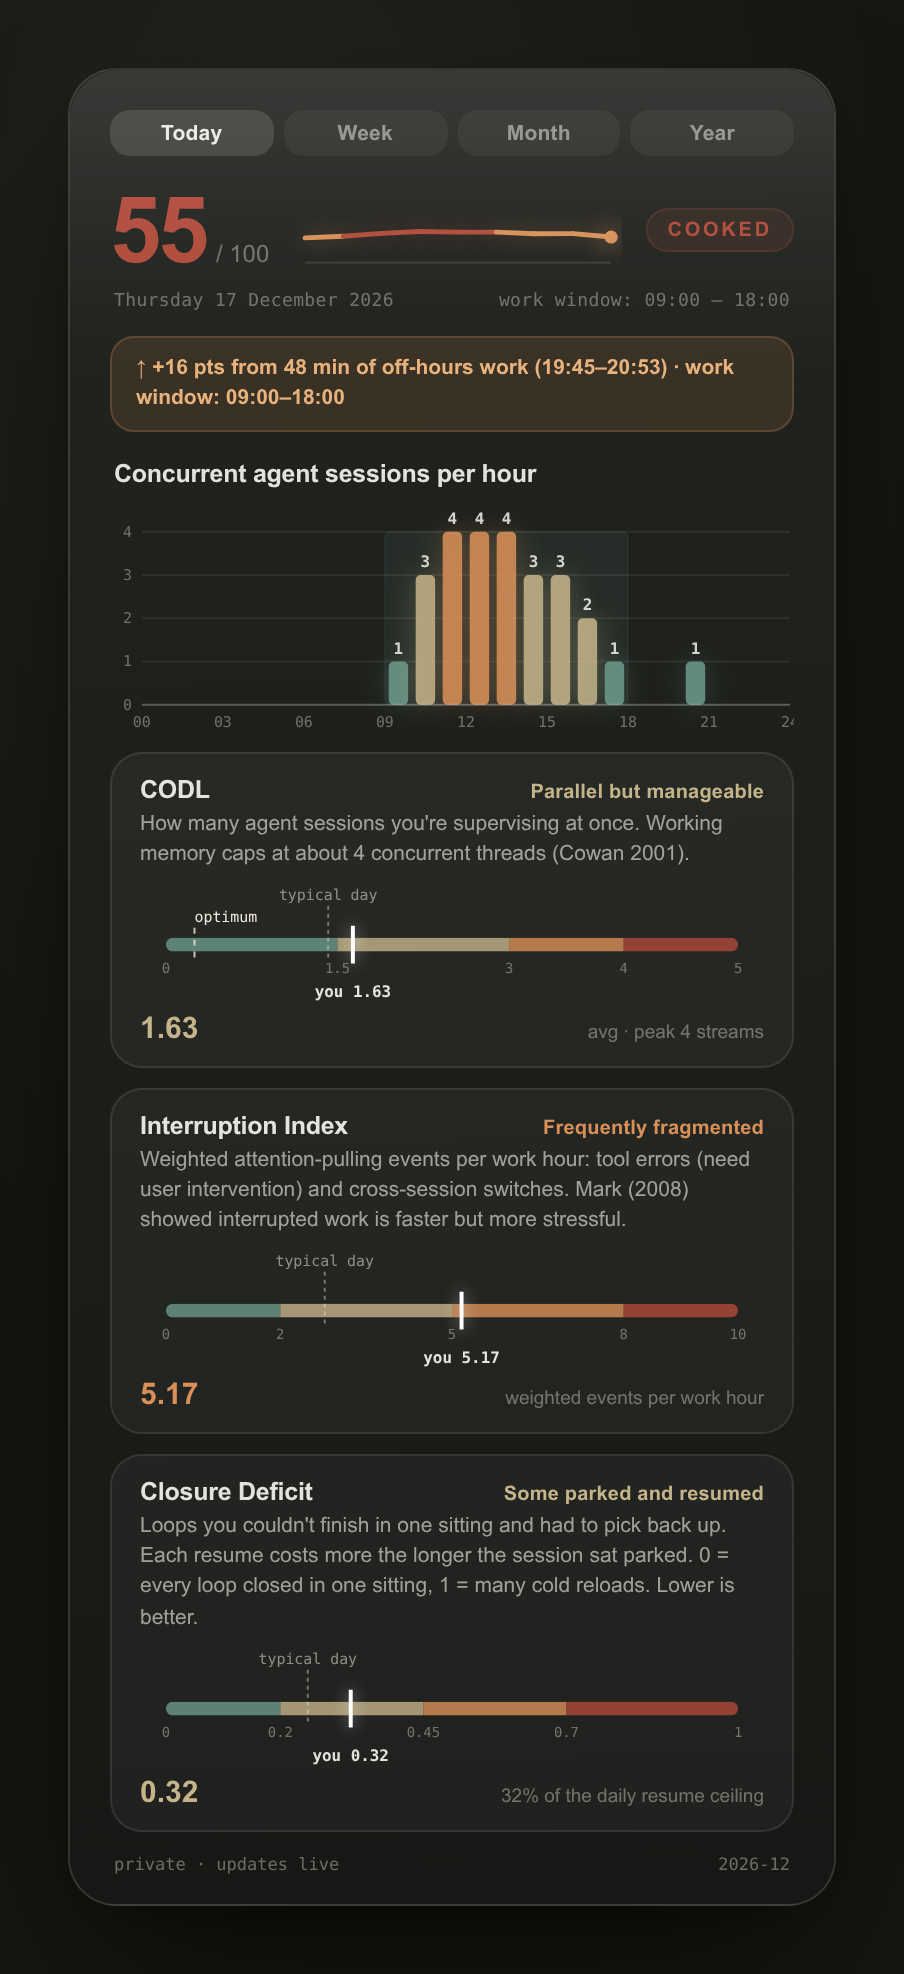
\includegraphics[height=6.4cm]{../docs/screenshots/widget-today.png}\hspace{3mm}
      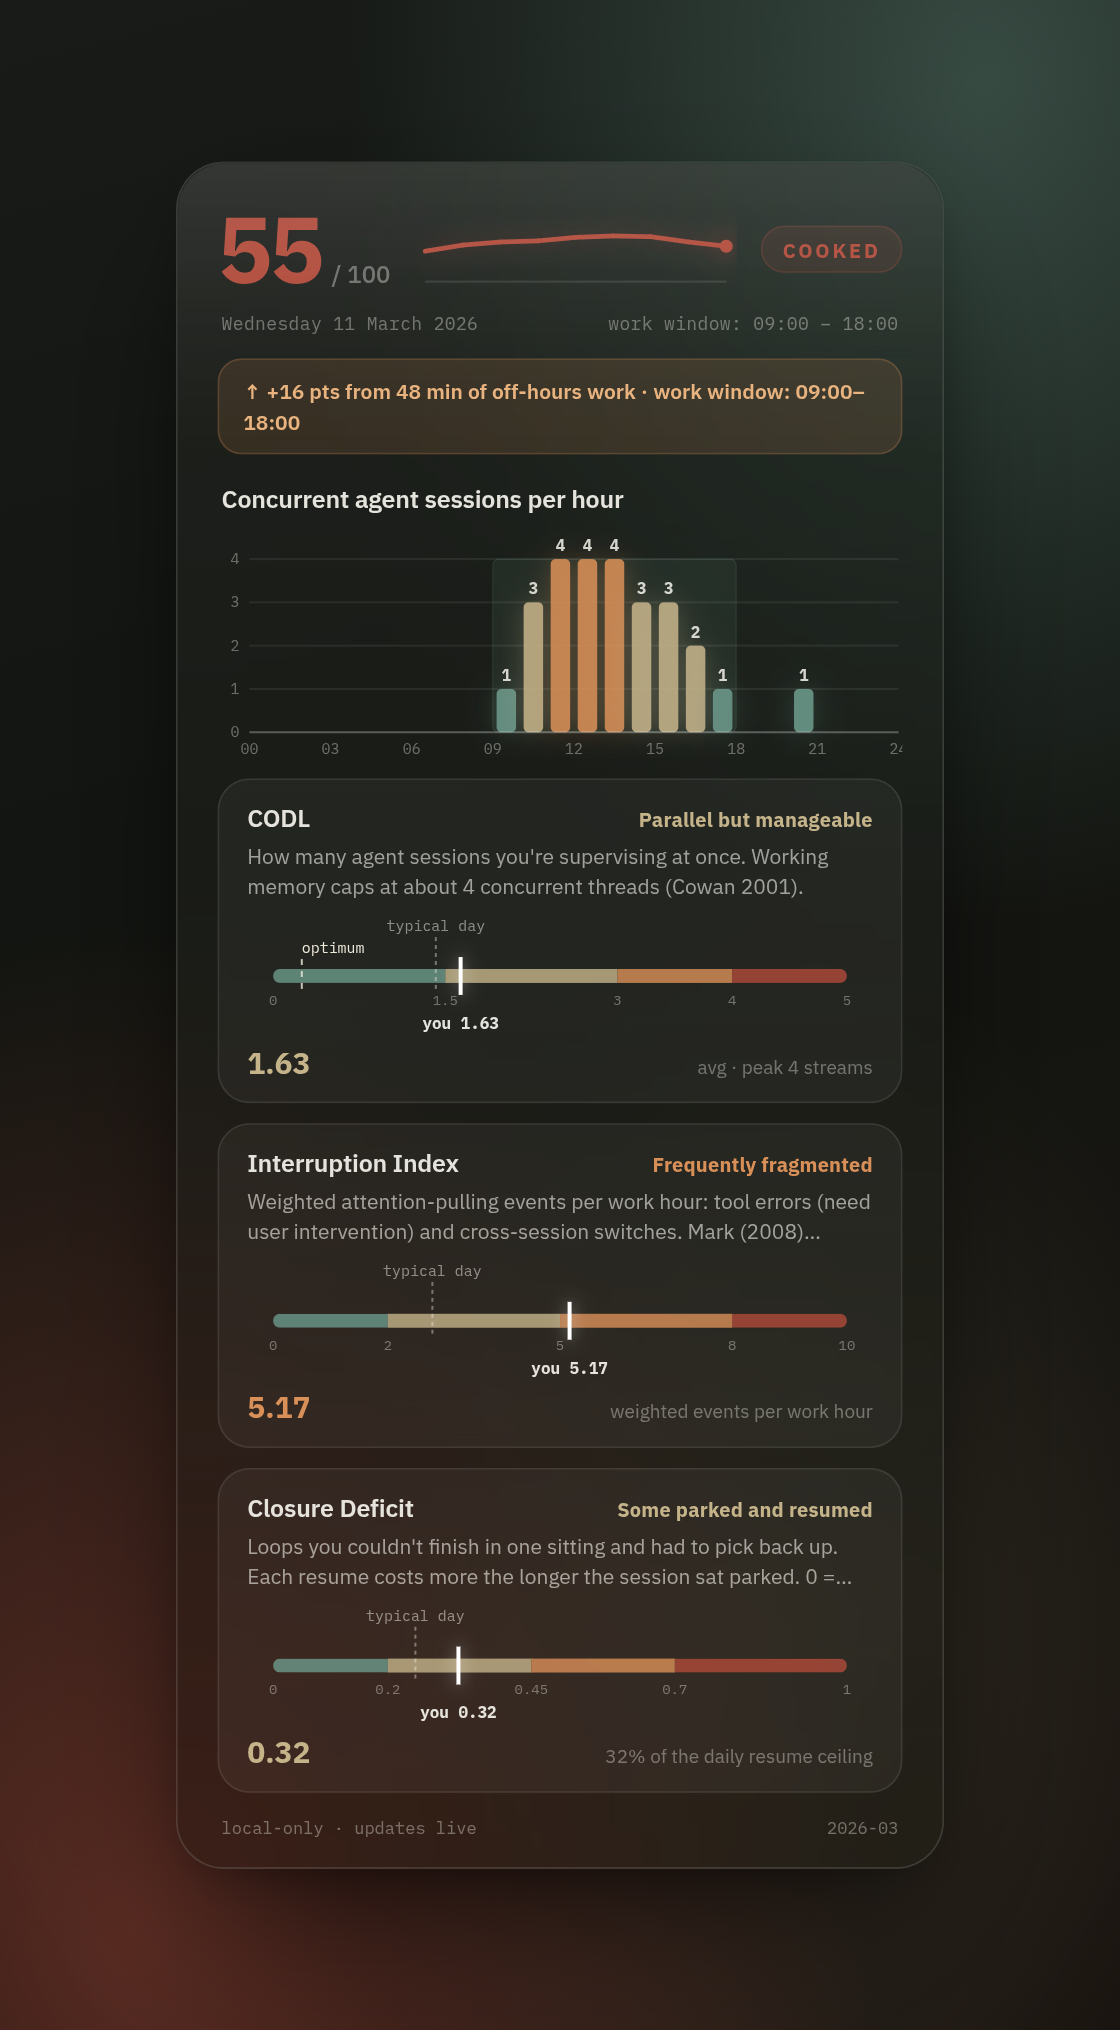
\includegraphics[height=6.4cm]{../docs/screenshots/ubersicht-widget.png}
    \end{column}
    \begin{column}{0.38\textwidth}
      \small
      \begin{itemize}
        \item One renderer produces a self-contained HTML card; thin hosts
              show it on KDE Plasma, any GTK desktop, macOS
              \"Ubersicht, and Windows.
        \item Today, week, month, and year tabs; a compact mini variant.
        \item The card is where the optional \good{felt-stress grade}
              (0--2) is entered: one action, stored locally, used only for
              calibration.
      \end{itemize}
    \end{column}
  \end{columns}
\end{frame}

% F21 · Privacy
\begin{frame}{Private by design}
  \begin{itemize}
    \item Session transcripts routinely contain \alert{proprietary code and
          secrets}; the generated report and JSON are treated as equally
          sensitive.
    \item The tool reads local files and writes local files:
          \good{no network calls at any stage}, no telemetry, no remote
          rendering. Privacy is a hard invariant, not a feature toggle.
    \item Intended use is \good{individual self-assessment}. The index is
          calibrated to one person's history; using an unvalidated load
          proxy to evaluate people would be statistically and ethically
          unsound, and the paper says so explicitly.
  \end{itemize}
  \vspace{2mm}
  \begin{beamercolorbox}[rounded=true,sep=6pt]{block body}
    \footnotesize\texttt{git clone \repourl{}\\
    cd ai-code-cognitive-stress \&\& python3 install.py \&\& aicogstress -{}-open}
  \end{beamercolorbox}
\end{frame}

% =========================================================================
\section{The research, honestly}
% =========================================================================

% F22 · What it is not
\begin{frame}{What this is, and what it is not}
  \begin{columns}[T]
    \begin{column}{0.48\textwidth}
      {\small\good{It is}\par}
      \begin{itemize}
        \item an objective, behavioural \good{taskload proxy}, computed
              continuously from real sessions;
        \item longitudinal and per-person: only relative movement within
              one's own history is interpreted;
        \item fully open: every threshold is an explicit, cited,
              configurable prior.
      \end{itemize}
    \end{column}
    \begin{column}{0.48\textwidth}
      {\small\badc{It is not}\par}
      \begin{itemize}
        \item a measure of \emph{felt} workload: that is NASA-TLX;
              \src{Hart \& Staveland (1988).}
        \item a burnout diagnosis: that is the MBI;
              \src{Maslach \& Jackson (1981).}
        \item validated yet: thresholds are borrowed from adjacent
              literature, and no field data is reported; the illustrative
              example ships on synthetic sample data.
      \end{itemize}
    \end{column}
  \end{columns}
  \vspace{2mm}
  {\small The paper attacks its own construct in an eleven-item threats
   section and states \good{falsifiable predictions}: if the three axes
   predict felt load no better than a stopwatch, the decomposition should be
   simplified away.\par}
\end{frame}

% F23 · Reflexive loop
\begin{frame}{A paper that reviews its own code}
  \begin{columns}[T]
    \begin{column}{0.50\textwidth}
      \small
      \begin{itemize}
        \item The paper and the implementation \good{co-evolve}: each
              self-critique is treated as an adversarial review of the code
              \emph{and} of the premise behind an axis.
        \item A critique is first verified against the \emph{running} code;
              then the code is improved, or the paper corrected, or both.
        \item Two human gates bracket every change: plan approval and
              merged-diff review. Tests must stay green.
        \item Reflexivity: a paper about supervising coding agents,
              produced by supervising coding agents.
      \end{itemize}
    \end{column}
    \begin{column}{0.48\textwidth}
      \centering
      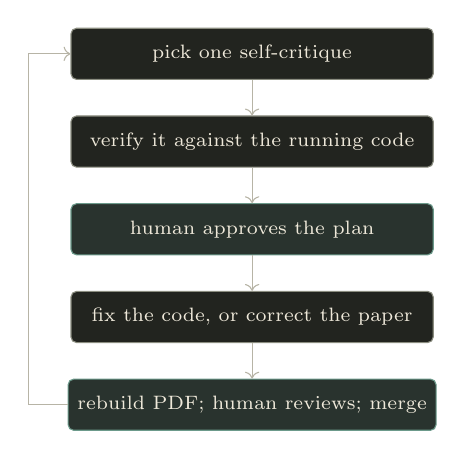
\begin{tikzpicture}[
        node distance=4.5mm,
        stage/.style={draw=InkFaint, fill=Panel, rounded corners=2pt,
                      text=Ink, font=\scriptsize, align=center,
                      minimum width=4.6cm, minimum height=6.5mm},
        gate/.style={stage, draw=Sage, fill=Sage!18!SlideBg}
      ]
        \node[stage] (crit) {pick one self-critique};
        \node[stage, below=of crit] (verify) {verify it against the running code};
        \node[gate,  below=of verify] (plan) {human approves the plan};
        \node[stage, below=of plan] (fix) {fix the code, or correct the paper};
        \node[gate,  below=of fix] (merge) {rebuild PDF; human reviews; merge};
        \draw[->, InkSoft] (crit) -- (verify);
        \draw[->, InkSoft] (verify) -- (plan);
        \draw[->, InkSoft] (plan) -- (fix);
        \draw[->, InkSoft] (fix) -- (merge);
        \draw[->, InkSoft] (merge.west) -- ++(-5mm,0) |- (crit.west);
      \end{tikzpicture}
    \end{column}
  \end{columns}
\end{frame}

% F24 · What data enables
\begin{frame}{The missing ingredient is a population}
  \begin{columns}[T]
    \begin{column}{0.50\textwidth}
      {\small\good{What pooled, anonymized exports enable}\par}
      \begin{itemize}
        \item Refit the axis \emph{scales} (dose horizon, interruption
              ceiling) to how agent-coding engineers actually behave.
        \item Check the borrowed anchors: Cowan's $\kappa\approx4$, the
              10/hour ceiling, $\beta=0.20$.
        \item With optional felt-stress grades: correlate each axis with
              felt load, and fit composite weights that must beat the
              equal-weight null \emph{out of sample}.
      \end{itemize}
    \end{column}
    \begin{column}{0.48\textwidth}
      {\small\good{What an export contains}\par}
      \begin{itemize}
        \item Derived daily metrics only: \badc{no code, no file paths, no
              usernames, no prompts}.
        \item Timezone dropped; calendar dates \good{randomly shifted}.
        \item Optionally, your coarse 0--2 felt-stress grades.
        \item Written to a \good{local file}; you inspect it and upload it
              \good{manually}. The tool itself transmits nothing.
      \end{itemize}
    \end{column}
  \end{columns}
  \vspace{2mm}
  {\small As contributions accrue, population baselines flow \good{back into
   the tool}, so every contributor sees how their patterns compare to the
   community.\par}
\end{frame}

% F25 · CTA
\begin{frame}{Three ways to help}
  \begin{columns}[T]
    \begin{column}{0.70\textwidth}
      \begin{enumerate}
        \item {\large\good{Use it.}} \small Clone the repo and ask your
              coding agent to install it: about a minute, and the report
              stays on your machine.\\
              {\footnotesize\texttt{git clone \repourl}}\\[7pt]
        \item {\large\good{Fork it.}} \small MIT-licensed, stdlib-only.\\[7pt]
        \item {\large\good{Contribute your anonymized data.}} \small Run
              \texttt{/contribute-data} in your coding agent: it writes the
              anonymized export locally and walks you through the manual
              upload.
      \end{enumerate}
    \end{column}
    \begin{column}{0.26\textwidth}
      \centering
      \setlength{\fboxsep}{6pt}%
      \colorbox{Ink}{\color{SlideBg}\qrcode[height=2.5cm]{\repourl}}\\[2mm]
      {\scriptsize\color{Sage}\url{\repourl}}
    \end{column}
  \end{columns}
\end{frame}

\end{document}
